\section{Results}
\label{sec:Results}
% Chaos
Plotting the probability of chaos against the competition parameter (see figure \ref{fig:Results}), we observe a clear maximum around $ \epsilon = 0 $. The likelihood of chaotic behaviour for neutral competition at the prey's trophic level is thus higher than for dominant inter or intraspecific competition. This result remains true for systems with a different number of species (figures \ref{fig:Results} and \ref{fig:Contour}).

The overall likelihood of chaos, which can be interpreted as the area under the curve in figure \ref{fig:Results}, increases with the size of the food web. This effect should not be surprising: the more dimensions the phase space has, the easier is to fulfill the requirements of the complex geometry of a chaotic attractor \citep{Strogatz1994}. Even in those higher dimensional cases, there is still a clear maximum at neutral competition. Another local maximum was observed for low values of $ \epsilon $, meaning that weak competitive coupling also promotes chaos in our model.

\begin{figure}
	\begin{center}
		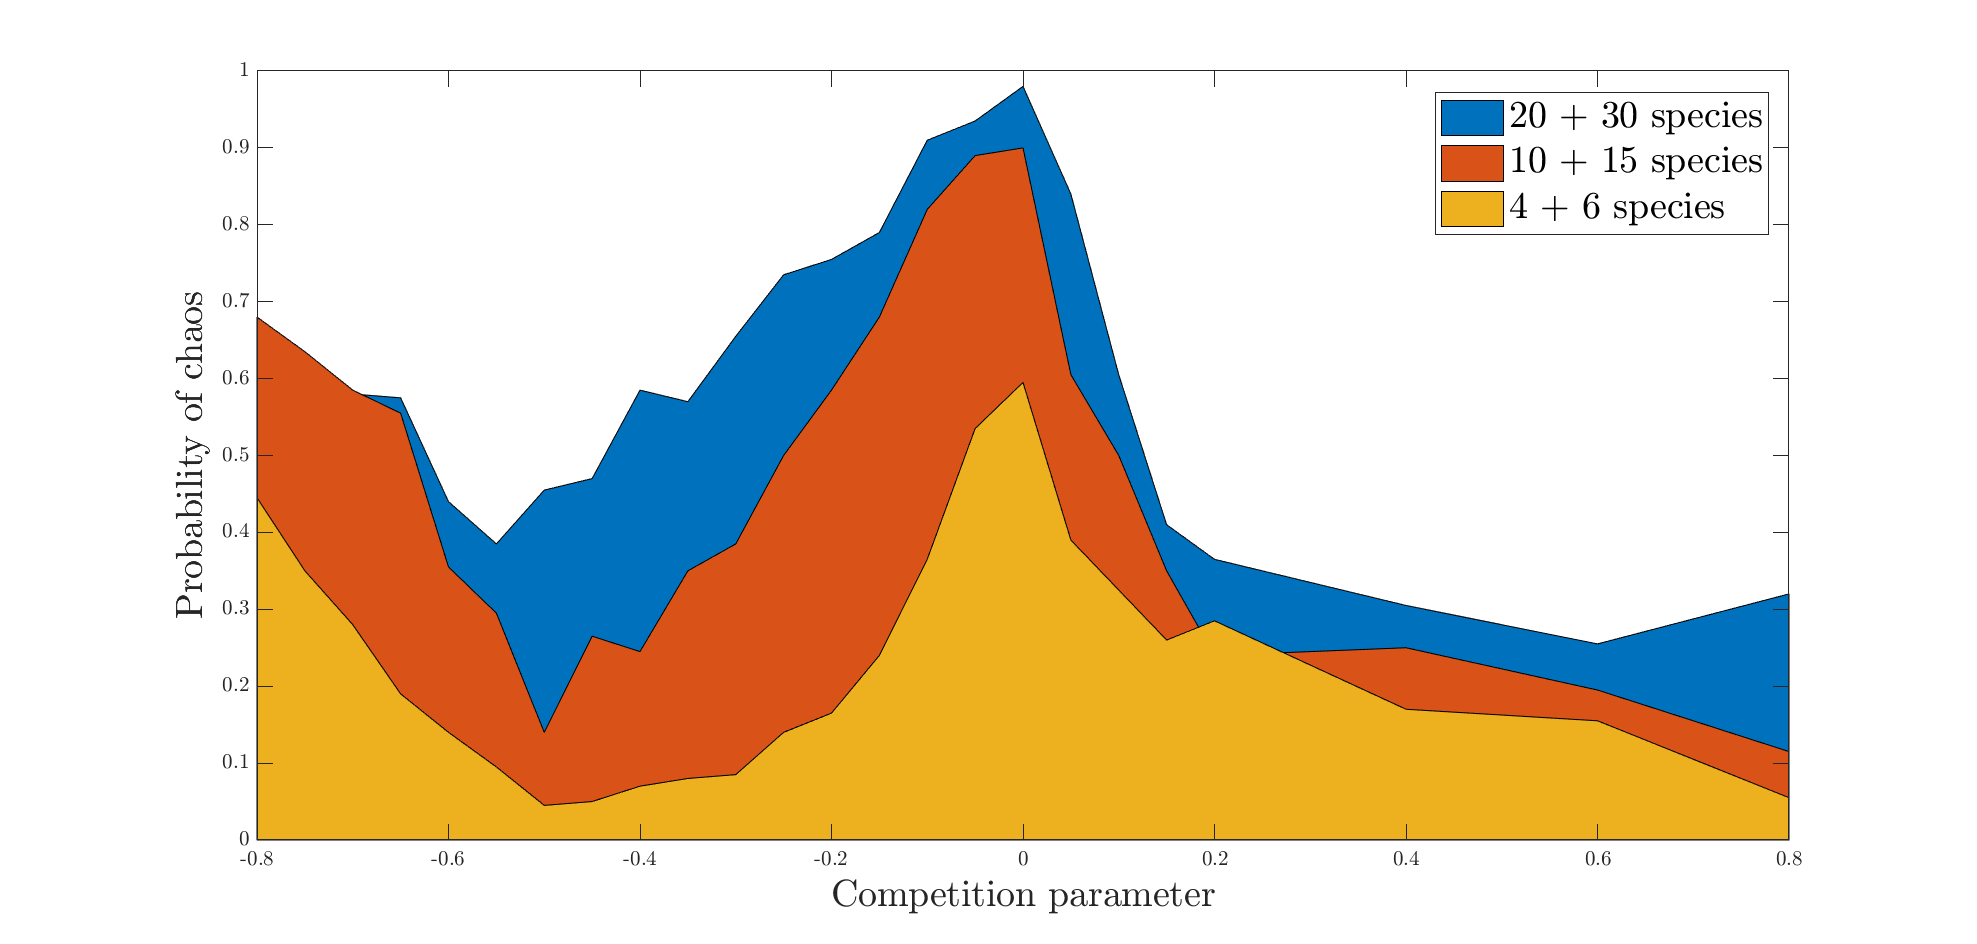
\includegraphics[width=1\columnwidth]{results.png}
	\end{center}
	\caption{Results for a low, medium and high dimensional system. The size of the food web is specified as number of predator species + number of prey species. The probability of chaos has a local maximum around $\epsilon = 0$. The effect remains true for food webs with different number of species. The overall probability of chaos, understood as the area under the curve, grows with the system size. }
	\label{fig:Results}
\end{figure}

\begin{figure}
	\begin{center}
		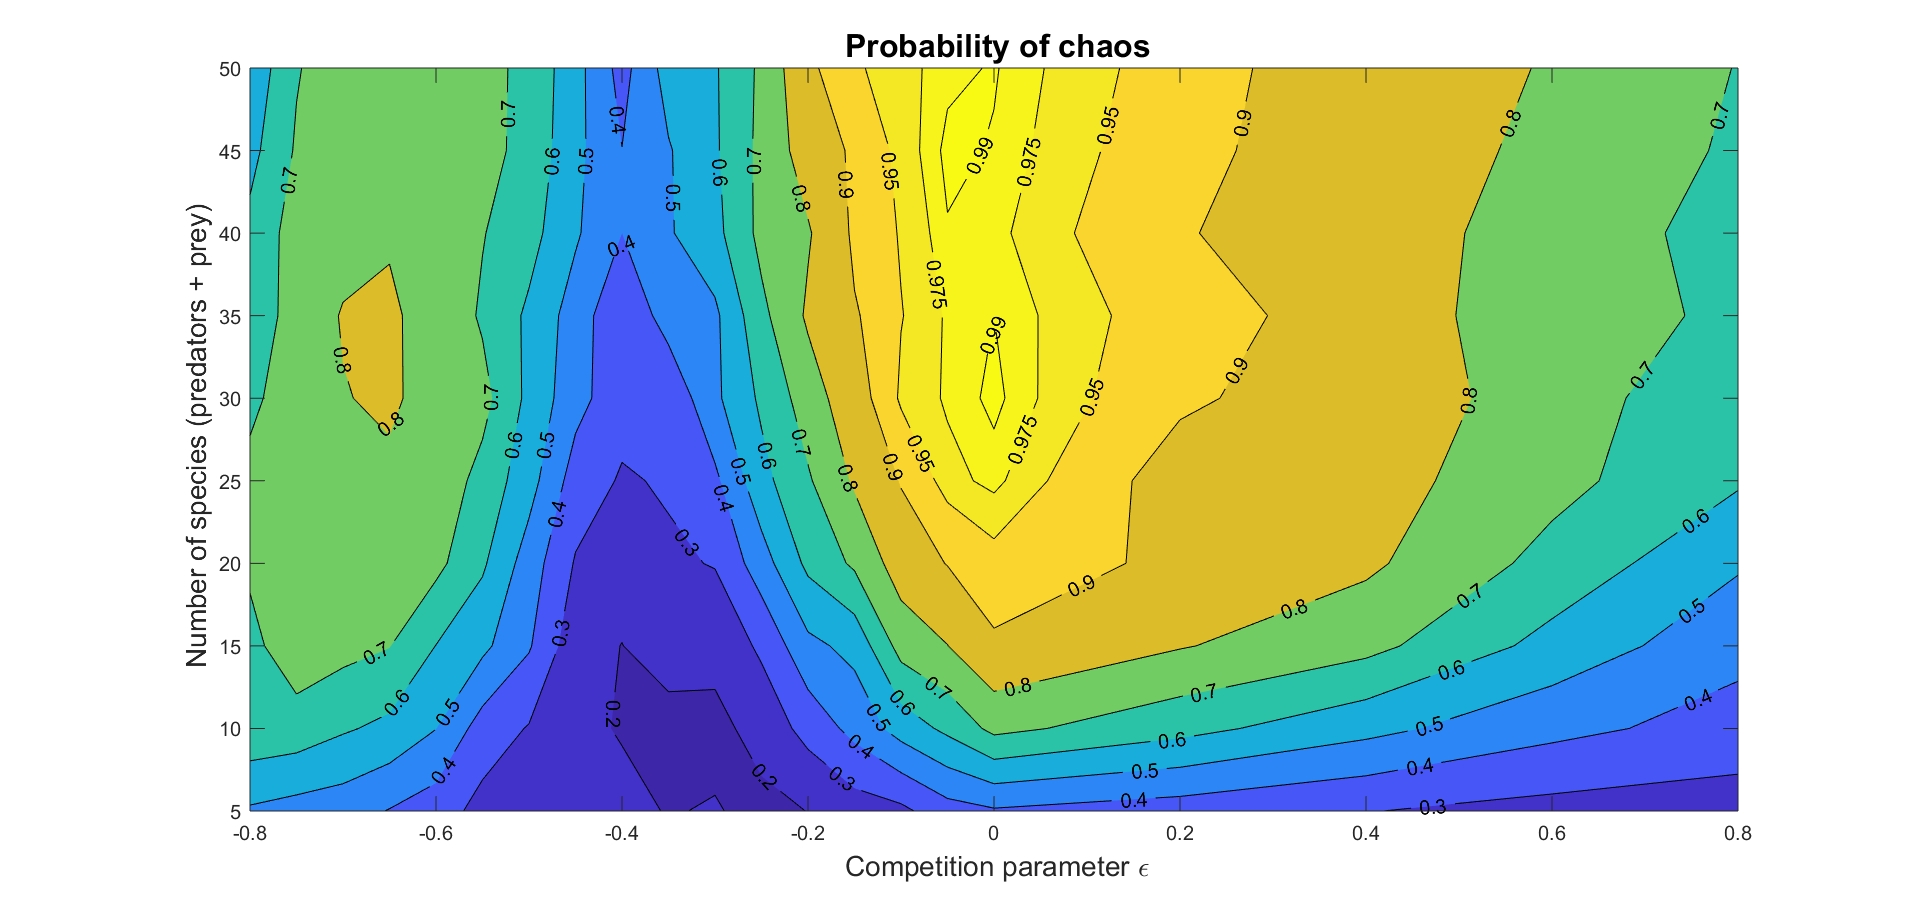
\includegraphics[width=1\columnwidth]{contour.png}
	\end{center}
	\caption{Contour map showing the probability of chaos for various competition parameters (horizontal axis) and number of species (vertical axis). The consumers' population is fixed as $ 2/3 $ of the prey's population. Notice that chaotic attractors appear more easily (i.e., for smaller systems) the closer is the competition to neutral (i.e., $ \epsilon = 0 $).}
	\label{fig:Contour}
\end{figure}

% Biodiversity
Our biodiversity measures (see figure \ref{fig:Biodiversity}) illustrate two effects: chaos clearly tends to increase biodiversity in our model and overall biodiversity is very close to its maximum around neutrality.

\begin{figure}
	\begin{center}
		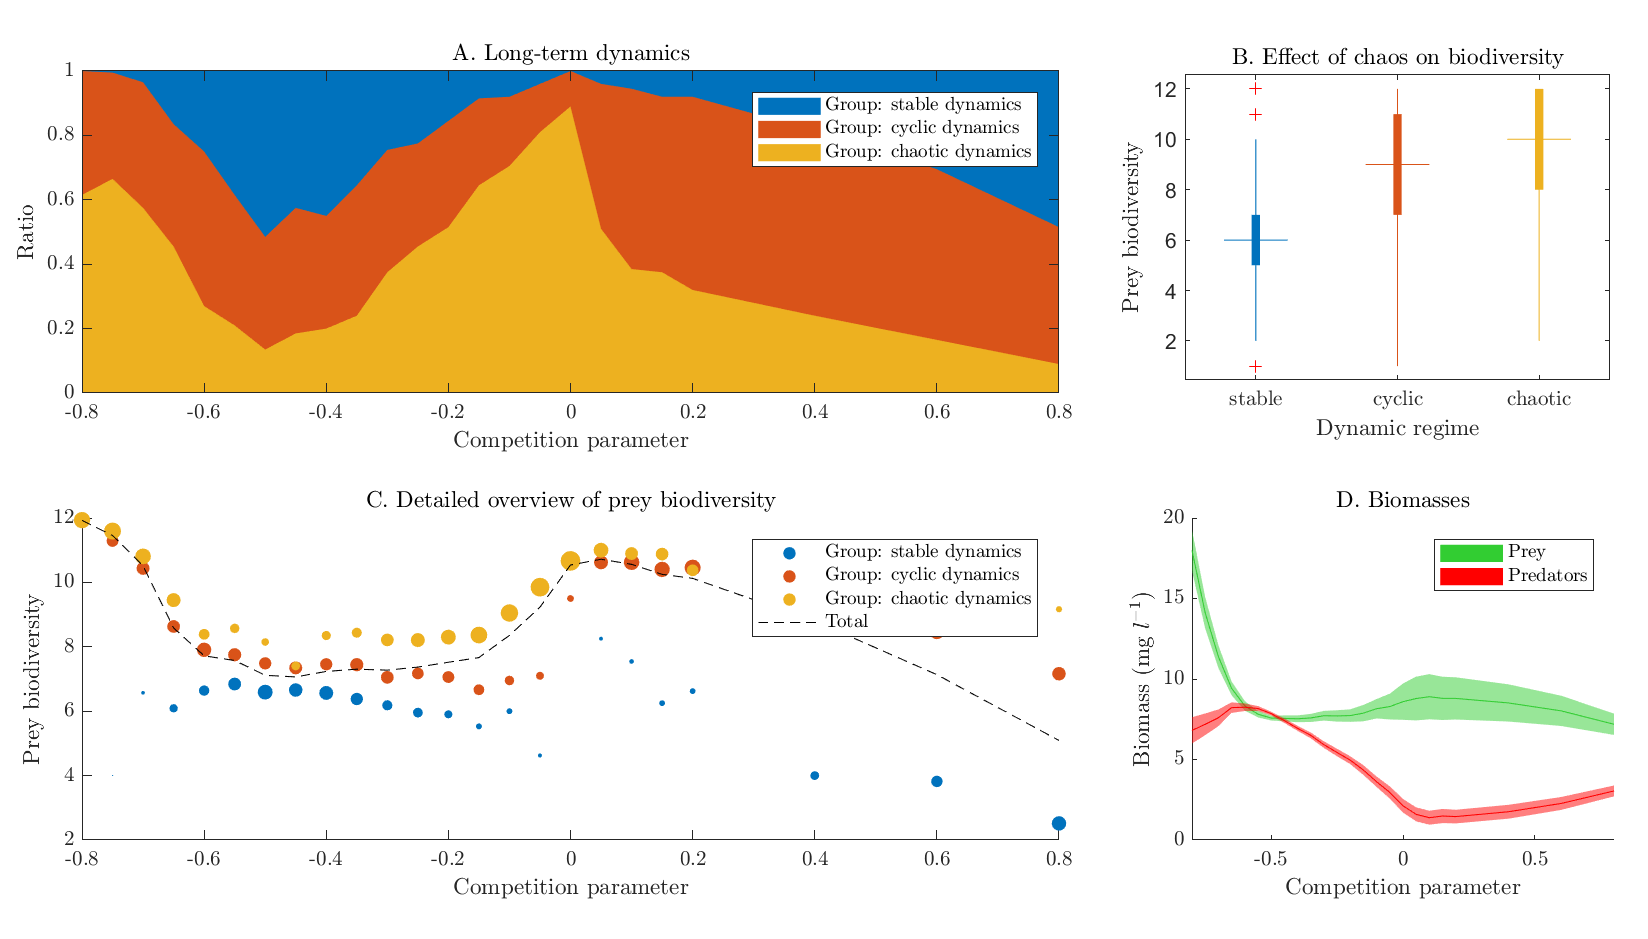
\includegraphics[width=1\columnwidth]{best.png}
	\end{center}
	\caption{Results for a food web with $10$ predator and $15$ prey species. Food webs of different sizes are qualitatively equivalent (see \ref{subsec:ExtraFigures} in Online Appendix). For each value of the competition parameter, $\numReps$ randomly drawn ecosystems were simulated and classified as regular or chaotic. Additionally, the number of non-extinct prey species after an stabilization run was registered. \textbf{Panel A} Probability of chaos vs. competition parameter. The proportion of ecosystems tagged as chaotic was used as an estimator of the probability of chaos. \textbf{Panel B} Average prey biodiversity vs. competition parameter. The dashed line shows the average number of non-extinct prey species grouped by competition parameter. The black and white circles represent the average prey biodiversity of the simulations, additionally grouped by the type of asymptotic dynamics (regular and chaotic, respectively). The relative size of the black and white circles represents the proportion of simulations that led to regular or chaotic dynamics. \textbf{Panel C} Biodiversity vs. asymptotic regime. Box and whisker plot of the number of non-extinct prey species grouped by asymptotic regime, regardless of the competition parameter.}
	\label{fig:Biodiversity}
\end{figure}